\documentclass{article}
\usepackage{ctex}
\usepackage{geometry}
\usepackage{amsfonts,amssymb}
\usepackage{listings} 
\usepackage{fontspec}
\usepackage{graphicx}
\geometry{a4paper,left=2.5cm,right=2.5cm,top=2cm,bottom=2cm}
\renewcommand{\baselinestretch}{1.5}
\title{科学计算作业1}	
\author{张文涛 517030910425}
\date{\today}
\lstset{columns=flexible,numbers=left,numberstyle=\tiny,basicstyle=\small,keywordstyle=\color{blue!70},commentstyle=\color{red!50!green!50!blue!50}, rulesepcolor= \color{ red!20!green!20!blue!20} }
\begin{document}
	\begin{itemize}
		\item[1.]给定函数$z = f(x, y) = x^{2}sin(y) + cos(x)y^{2}$,以及向量$x =[x_{1}, x_{2}, \cdots, x_{m}]^{T}$和$x =[y_{1}, y_{2}, \cdots, y_{n}]^{T}$,写一个MATLAB函数使得通过矩阵运算获得矩阵$Z = [z_{ij}]_{m\times n}$,式中$z_{ij} = f(x_{i}, y_{i})$,并画出该二元函数相应的曲面图。\\\\
		\begin{lstlisting}
		function A = calc(p, q);
		[x, y] = meshgrid(p, q);
		A = (x'.^2).*sin(y')+(y'.^2).*cos(x');
		surf(x',y',A), shading interp; colorbar
		\end{lstlisting}
		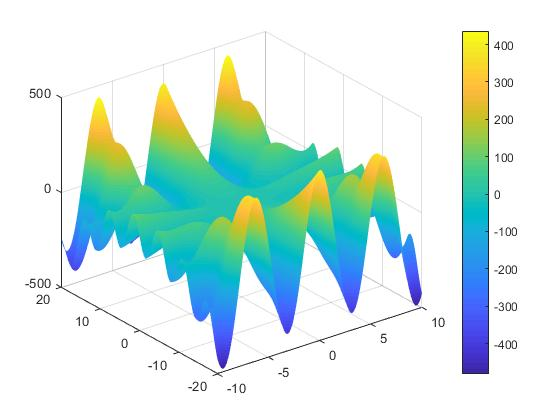
\includegraphics[scale=0.8]{HW1-GAI.jpg}
	\end{itemize}
\end{document}